% !TEX root = ../root.tex

\section{Sequential Circuits}
\firstthought{All of the circuits} we have considered so far have been acyclic; this was an essential part of the definition of a combinational circuit. In general, if a circuit has a cycle, its output behavior might not be well-behaved---consider the simple example of a \textsc{not} gate whose output feeds back to its input, so that if the output went high, it would be forced low after one gate delay, then back high after another delay, \textit{etc}.\footnote{In fact, since a physical device can only be an approximation of a pure logic gate, it is more likely that the output would hover around some intermediate level, neither high nor low.}

In this section, we will explore two ways of adding cycles to circuits in a controlled fashion. The first, operating on the level of just a few gates, will give us circuit components with memory. The second, using larger-scale feedback on circuits that include both combinational and memory components, will give us a means of implementing state machines and, ultimately, general-purpose processors. On the larger scale, the circuits will be what are known as ``synchronous''---that is, a clock signal is used to synchronize the times at which feedback is applied. At the small scale, we will start with ``asynchronous'' circuits, where feedback may arrive as soon as the gate delays permit. While it is possible to design large-scale asynchronous circuits, we will not be considering that here.

Circuits with cycles are known as ``sequential logic'' circuits, because the output depends on the particular \emph{sequence} of inputs the device has received in the past; unlike combinational circuits, the output is not solely determined by the current combination of input values but potentially by the entire history of inputs (in other words, it is not purely functional---its behavior depends on side-effects). As a result, they can be considerably harder to reason about, and we will need good abstract models, such as state machines.

\subsection{Memory Devices}
\firstthought{Although the circuit} with one \textsc{not} gate feeding back on itself is unstable, a cycle of two \textsc{not} gates would be fine:
\begin{center}
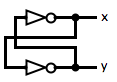
\includegraphics[width=!,height=!,scale=0.75]{NotLatch.png}
\end{center}
Whatever the output is at $x$, the output at $y$ will be the opposite. Each one feeds back and reinforces the other, and the circuit is stable. Unfortunately, it is not very useful---there is no way to provide input to \emph{change} the value $x$.

By replacing the \textsc{not} gates with either \textsc{nand} or \textsc{nor} gates, we get a circuit known as a latch. Here is the diagram for a so-called $\overline{SR}$ latch:
\begin{center}
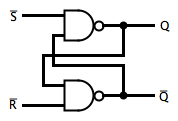
\includegraphics[width=!,height=!,scale=0.75]{SRLatch.png}
\end{center}
When the inputs $\overline{S}$ (set) and $\overline{R}$ (reset) are both \1, the latch behaves just like the circuit with two \textsc{not} gates (because $\1\uparrow x=\overline{x}$): whatever the output is at $Q$, the opposite value will be at $\overline{Q}$ (hence its customary label---it is the negation of $Q$).

When the $\overline{S}$ input is \0, the output $Q$ is forced to \1---the latch is ``set'' (the label $\overline{S}$ suggests that it is ``active-low'': the latch will be set when the input is false). Again, because of the feedback, when $Q$ is \1, $\overline{Q}$ will be \0. Returning $\overline{S}$ to \1 \emph{will then leave the latch in the set state}. This is where the sequential nature of the latch shows: its state depends on its past history (in this case, the fact that the set line was most recently active).

When the $\overline{R}$ input is \0, the output $\overline{Q}$ is forced to \1 and correspondingly $Q$ will become \0---the latch has been ``reset.'' Again, returning $\overline{R}$ to \1 will leave it in the reset state, until the set line is next activated.

If both the set and reset lines are active (\0), then both output lines will be forced to \1. This presents two problems: it violates the property that $Q$ and $\overline{Q}$ are complementary, and it sets up a potential race condition if both lines are restored to \1 at the same time. When the inputs are \1, exactly one of the outputs can be high; however, which one ``wins'' the race will depend on the precise timing of the transitions from \0 to \1, and potentially also on slight imperfections in the gates (if one of the \textsc{nand} gates responds slightly faster than the other, for example). So, don't do that.

The $\overline{SR}$ latch is what is known as a \textit{transparent} latch: the output responds as soon as the input is changed. To make sequential design easier, we frequently want memory devices that will only respond at certain times. By adding an extra layer of gates to the input, we can make what is known as a ``gated D latch.'' The inputs are $D$ (data) and $E$ (enable):
\begin{center}
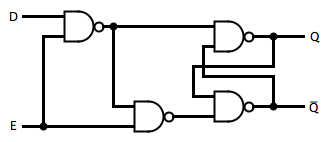
\includegraphics[width=!,height=!,scale=0.75]{DELatch.png}
\end{center}
As long as $E$ is \0 (note that this is now an active-high device), the $\overline{S}$ and $\overline{R}$ inputs to the latch will always be \1, regardless of the $D$ input. The gated D latch is only enabled when the $E$ input is \1. When enabled, the latch becomes transparent: if $D$ is \1, then $\overline{S}$ will be \0, and the output $Q$ will be set to \1; if $D$ goes to \0, then $\overline{R}$ will be \0 and the latch will be reset. There is no combination of inputs for $D$ and $E$ which can make both the set and reset lines active at the same time, so we don't have to worry about that case.

When the enable line returns to \0, the gated D latch will remain in whatever state it last entered. Here is a truth table for the latch, together with its common symbol when used in a circuit:
\[ \begin{array}[b]{cc|cc}
E & D & Q & \overline{Q}\\ \hline
\0 & X & \multicolumn{2}{c}{\textrm{last state}}\\
\1 & \0 & \0 & \1\\
\1 & \1 & \1 & \0
\end{array}\hspace{1cm}
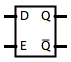
\includegraphics[width=!,height=!,scale=0.75]{DELatchSymbol.png}
\]

When dealing with a sequential circuit, it is often helpful to look at a \emph{timing diagram}, which shows the levels at various points of the circuit over time (increasing from left to right). Here is a timing diagram for the gated D latch, which shows that the output is transparent to the $D$ input only when $E$ is high:
\[ \begin{array}{cc}
E & \texttiming{2C2C2C2C}\\
D & \texttiming{LHLHLHLH}\\
Q & \texttiming{LLLHHHLH}
\end{array} \]

\newthought{Instead of a latch}, it is more common to use a device known as a ``flip-flop.'' The distinction from a latch is that a flip-flop will only respond to input for a very brief time; it is what is known as a \textit{clocked} device, since it will only change its state when a clock pulse is received (typically, just as the clock pulse is rising from \0 to \1). In \emph{synchronous} logic design, the entire circuit will use a single clock signal, so that each clock pulse advances the state by one step (and the state has time to propagate through all the gate delays before the next pulse). Here is one design for an edge-triggered D flip-flop:
\begin{center}
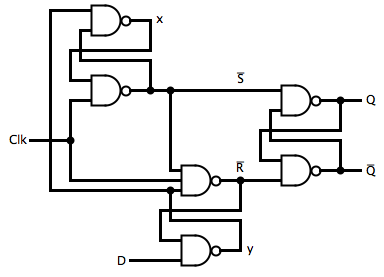
\includegraphics[width=!,height=!,scale=0.75]{DFlipFlop.png}
\end{center}
Just as the gated D latch modified an $\overline{SR}$ latch by adding a layer of two \textsc{nand} gates, this flip-flop modifies an $\overline{SR}$ latch by adding a layer of two input latches. In each case, the input layer protects the output latch from entering the illegal state (both $\overline{S}$ and $\overline{R}$ low).

The idea is that, as long as the clock (\textit{Clk}) is \0, the set ($\overline{S}$) and reset ($\overline{R}$) lines of the output latch will stay high (inactive). The line marked $x$ will be whatever $D$ is, and the line marked $y$ will be the opposite, $\overline{D}$. Although one of the input latches will be in an ``illegal'' state, the output latch will not be affected.

When the clock goes to \1, the input latches will resolve to consistent states: $\overline{S}$ will be $\overline{x}=\overline{D}$, and $\overline{R}$ will be $\overline{y}=D$. That is, if $D$ was \0, then the output latch will be reset, while if $D$ was \1 it will be set. However, once the clock reaches \1, further changes to $D$ will be ignored: if the lower input latch is reset ($\overline{R}$ is \0, meaning $D$ was \0 at the rising edge), then changing $D$ will leave it in the reset state; if instead the lower input latch is set ($\overline{R}$ is \1, meaning $D$ was \1 at the rising edge), then changing $D$ will switch it between the set and illegal states (where $\overline{R}$ is still \1), and the upper input latch will stay in the set state.

When the clock goes back to \0, the output latch will continue to hold whatever state it had (because both of its inputs will be \1 again), until the next time the clock rises.

The only danger with this design is if $D$ is changed at exactly the same time as the rising of the clock signal, because then if one of the input latches was in an illegal state it is possible to have a race condition. Designers avoid this by arranging for the $D$ input to be stable for at least a brief ``setup and hold'' time around clock pulses.

Here is a timing diagram for the D flip-flop, and its common circuit signal (the input marked with a triangle indicates that it is a rising-edge-triggered clock):
\[ \begin{array}[b]{rc}
\textit{Clk} & \texttiming{2C2C2C2C2C2C2C2C}\\
D & \texttiming{lLHLHLLLHHHLHLHHh}\\
Q & \texttiming{LLHHHHLLLLHHHHHH}
\end{array}\hspace{1cm}
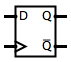
\includegraphics[width=!,height=!,scale=0.75]{DFlipFlopSymbol.png}
\]

Rather than a truth table, it is useful to give what are known as a \emph{characteristic table} or an \emph{excitation table} for a flip-flop. The characteristic table shows how the input ($D$) and current state ($Q$) lead to the next state ($Q'$) after the clock pulse:
\[ \begin{array}{cc|c}
D & Q & Q'\\ \hline
\0 & \0 & \0\\
\0 & \1 & \0\\
\1 & \0 & \1\\
\1 & \1 & \1
\end{array} \]
The excitation table presents the same information, but from the viewpoint of ``given a current state $Q$ and desired next state $Q'$, what does the input need to be?''
\[ \begin{array}{cc|c}
Q & Q' & D\\ \hline
\0 & \0 & \0\\
\0 & \1 & \1\\
\1 & \0 & \0\\
\1 & \1 & \1
\end{array} \]

\begin{tailquote}
The first electronic latch was the Eccles-Jordan trigger circuit. Patented in 1918, it was built out of two vacuum tubes connected in a feedback loop. In the early 1940's, Thomas Flowers (1905--1998) used his experience with telephone switching circuits to build Colossus, one of the code-breaking machines at Bletchley Park. The Colossus design used the Eccles-Jordan circuit as a storage register; it is considered the first programmable, electronic, digital computer, although its existence was kept secret until the 1970's.
\end{tailquote}
\begin{exercises}
\item Investigate the behavior of a latch built with \textsc{nor} gates instead of the \textsc{nand} gates used in the $\overline{SR}$ latch. Use this new latch to build a gated D latch.

\item There are several other types of flip-flops besides the D. Perhaps the most general is the JK flip-flop, which has two inputs, traditionally named $J$ and $K$, along with a clock input and the complementary $Q$ and $\overline{Q}$ outputs. When $J$ and $K$ are both \0 and a clock pulse arrives, the state does not change. When only $J$ is \1, the new state will be \1; when only $K$ is \1, the new state will be \0 (so $J$ \emph{sets} and $K$ \emph{resets} the flip-flop). Finally, when both $J$ and $K$ are \1, the clock pulse will cause the state to \emph{toggle}---that is, it will switch to the negation of its previous state. Here is the characteristic table of the JK flip-flop, using $X$ to indicate ``don't care'' inputs:
\[ \begin{array}{ccc|c}
J & K & Q & Q'\\ \hline
\0 & \0 & \0 & \0\\
\0 & \0 & \1 & \1\\
\0 & \1 & X & \0\\
\1 & \0 & X & \1\\
\1 & \1 & \0 & \1\\
\1 & \1 & \1 & \0
\end{array} \]
\begin{enumerate}
\item Draw a timing diagram that shows the behavior of the JK flip-flop.
\item Give an excitation table for the JK flip-flop.
\item Show how to construct a JK flip-flop using a D flip-flop plus a few extra gates. \textit{(Hint: Combine the $J$ and $K$ inputs with the current outputs $Q$ and $\overline{Q}$ to generate an appropriate $D$ input.)}
\end{enumerate}

\item Random-access memory (RAM) devices can be made from a quantity of flip-flops plus a few extra components such as multiplexers and demultiplexers. To store $2^k$ individually-addressable bits, you need one D type flip-flop per bit. The $D$ inputs can all be connected to an incoming data line; if each flip-flop's clock signal is driven by one line of a $k$-bit demultiplexer whose input signal is the \textsc{and} of the system clock signal and a ``write enable'' input, then the flip-flop selected by the $k$ address lines will be loaded with the desired data only if a write is enabled at the rise of the clock. Connecting the outputs of the flip-flops to a multiplexer, whose $k$ select lines are also driven by the $k$-bit address, will cause the contents of the selected bit to be passed to the output of the MUX. Use this description to draw a 16-bit RAM circuit, then show how to expand it to store four bits at each address.
\end{exercises}

\subsection{State Machines}
In Section~\ref{sec:moore} we learned about Moore machines, a version of finite state automata where there is an output associated with each state. Using flip-flops, we can build a circuit that implements a Moore machine. Here is a block diagram for such a circuit (although the connections are shown as single wires, all but the clock may be several bits wide):
\begin{center}
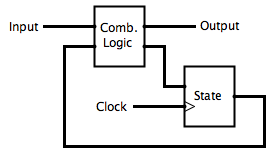
\includegraphics[width=!,height=!,scale=0.75]{MooreMachine.png}
\end{center}
In addition to the feedback within each flip-flop, there is a larger-scale feedback loop of the current state back to provide input for the next step. The box labelled ``Comb. Logic'' is a combinational circuit with two functions: compute an output based on the current state, and compute the next-state control signals based on the input and the current state. The box labelled ``State'' is one or more flip-flops; when a clock pulse arrives, it takes the control signals from the combinational logic and advances to the next state---the \emph{state} of the machine is simply the current states of these flip-flops.

If there are $k$ flip-flops, each of which can be \0 or \1, then the machine can be in $2^k$ different states. Therefore, if our Moore machine needs $n$ states, we will need at least $\lceil\lg n\rceil$ flip-flops. One step in designing the circuit for a given machine will be to assign a binary encoding to each state. For example, if the machine has three states, $A$, $B$, and $C$, then we will need two flip-flops. The circuit state will be the combination of the flip-flop outputs: $Q_1Q_0$. Given this, we may arbitrarily choose the encoding $A=\0\0$, $B=\0\1$, and $C=\1\0$ (and the state $\1\1$ will go unused).

Although the diagram shows the combinational logic has both the machine input and the current state available to compute the output, the convention in a Moore machine is that only the state is used to determine the output. There is a practical reason for this: during a clock cycle, as soon as the current state has propagated through the logic gates, we want the output to be available and stable. The input signals may not be stable until close to the end of the cycle (just before they are needed to determine the next state), and we would prefer not to see ``glitches'' in the output while the input might still be changing.

Here is an example of this process. Consider the following state machine for a mod-3 up/down counter:
\begin{center}
\begin{tikzpicture}[->,>=stealth',shorten >=1pt,auto,node distance=2.8cm,semithick]
  \node[initial,state](q0){$q_0/\0\0$};
  \node[state](q1)[right of=q0]{$q_1/\0\1$};
  \node[state](q2)[right of=q1]{$q_2/\1\0$};
  
  \path(q0) edge             node {\0} (q1)
            edge [bend left] node {\1} (q2)
       (q1) edge             node {\0} (q2)
            edge [bend left] node {\1} (q0)
       (q2) edge [bend left,in=120,out=60] node {\0} (q0)
            edge [bend left] node {\1} (q1);
\end{tikzpicture}
\end{center}
It has one input; call it $a$. When $a$ is \0, each clock pulse increments the counter through the states $q_0$, $q_1$, $q_2$, and back to $q_0$. When $a$ is \1, it decrements. At each state, the output is the corresponding number in binary: \0\0, \0\1, and \1\0.

We will use two D flip-flops, and the obvious encoding of states to bit patterns (which also happens to be the mapping from state to output, so we can just use the current state, \0\0, \0\1, or \1\0, to drive the output directly). All that remains is to design the combinational circuit that computes the $D_1$ and $D_0$ flip-flop control signals based on the input and current state. For this, we will first fill in a truth table with current state, input, and desired next state values, then use the excitation table for the flip-flops to decide an appropriate signal (for type-D flip-flops, this is particularly easy, since the required $D$ input is just the next state $Q'$):
\[ \begin{array}{ccc|cc|cc}
\multicolumn{2}{c}{\textit{current}} & \textit{input} &
  \multicolumn{2}{c}{\textit{next}} & \multicolumn{2}{c}{\textit{control}}\\
Q_1 & Q_0 & a & Q_1' & Q_0' & D_1 & D_0\\ \hline
\0 & \0 & \0 & \0 & \1 & \0 & \1\\
\0 & \0 & \1 & \1 & \0 & \1 & \0\\
\0 & \1 & \0 & \1 & \0 & \1 & \0\\
\0 & \1 & \1 & \0 & \0 & \0 & \0\\
\1 & \0 & \0 & \0 & \0 & \0 & \0\\
\1 & \0 & \1 & \0 & \1 & \0 & \1
\end{array} \]
Here is the Karnaugh map for $D_1$:
\[ \begin{array}{r|cccc}
& \overline{Q}_1\overline{Q}_0 & \overline{Q}_1Q_0 & Q_1Q_0 & Q_1\overline{Q}_0\\ \hline
\overline{a} & \0 & \tikzmark{left2}\1 & X\tikzmark{right2} & \0\\
a & \tikzmark{left1}\1\tikzmark{right1} & \0 & X & \0
\end{array}
\DrawBox[blue]{left1}{right1}
\DrawBox[red]{left2}{right2} \]
And here is the map for $D_0$:
\[ \begin{array}{r|cccc}
& \overline{Q}_1\overline{Q}_0 & \overline{Q}_1Q_0 & Q_1Q_0 & Q_1\overline{Q}_0\\ \hline
\overline{a} & \tikzmark{left1}\1\tikzmark{right1} & \0 & X & \0\\
a & \0 & \0 & \tikzmark{left2}X & \1\tikzmark{right2}
\end{array}
\DrawBox[blue]{left1}{right1}
\DrawBox[red]{left2}{right2} \]
Therefore, simple DNF expressions for the control signals are $D_1=\overline{Q}_1\overline{Q}_0a+Q_0\overline{a}$ and $D_0=\overline{Q}_1\overline{Q}_0\overline{a}+Q_1a$. The full circuit for the counter is given in Figure~\ref{fig:Mod3Counter}.
\begin{figure}
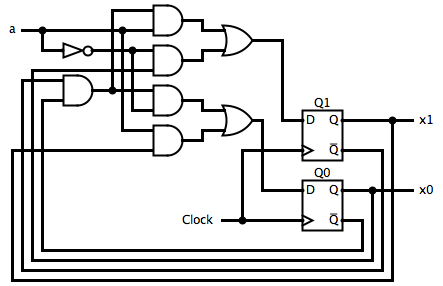
\includegraphics[width=!,height=!,scale=0.75]{Mod3Counter.png}
\caption{State machine circuit for a mod-3 up/down counter}
\label{fig:Mod3Counter}
\end{figure}

\begin{tailquote}
With combinational circuits to perform arithmetic and logic operations on data, plus registers to store intermediate results and keep track of program steps, a sequential circuit allows us to model an entire central processing unit. By connecting the inputs and outputs to external storage and I/O devices, the CPU forms the core of a general-purpose computer; details are left to the reader.
\end{tailquote}
\begin{exercises}
\item Design a BCD accumulator whose input is a three-bit two's complement number representing the value to be added to the total. That is, the state will be a decimal digit 0--9, represented in binary (\0\0\0\0 through \1\0\0\1). The output should be the signal lines to drive a seven-segment display (see Exercise~\ref{ex:BCD} of Section~\ref{sec:circsimp}). If the input is \0\0\0, then the state will be unchanged. If the input is +1 (\0\0\1) through +3 (\0\1\1), then that number will be added on each clock pulse. If the input is -4 (\1\0\0) through -1 (\1\1\1), then the total will go down by that amount on each pulse.

\item Reinterpret the block diagram for a Moore machine to produce a Mealy machine, where an output is associated with each transition. That is, the output should be determined by the current state \emph{and} the input. What might happen to the output if the input changes during a clock cycle? Compare this behavior to a Moore machine.
\end{exercises}


